% !TEX root = ../main.tex

\documentclass[../main.tex]{subfiles}
\begin{document}

Entering the 2010, machine learning and non-symbolic approaches had begun to capture the market, both in research and in commercial applications. In the previous section, we stressed how the absolute most relevant, impactful and impressive advance was in fact the \textit{availability} of large-scale datasets. Here, we will see what this caused, and what the current state-of-the-art is able to do. We will also use this opportunity to consider what the level of expertise required is, and briefly describe the two main frameworks for creating and training deep learning networks.

Before reading on, if you do not have experience with basic machine learning and neural networks, we ask you to read Appendix A. This content was moved to an appendix not because of its secondary importance, but only to avoid making this chapter too long. In what follows, Appendix content won't be re-introduced.

\subsection{AI}
Throughout the recent years, the AI field has boomed, in no small part thanks to deep learning's success. Wikipedia points to the ``big bang" of deep learning as early as 2009, when researchers started training deep learning neural networks on Nvidia GPUs. Others\cite{parloffWhyDeepLearning2016} point to the ImageNet victory in late 2012, or a related paper a couple months prior\cite{ciresanMulticolumnDeepNeural2012}, but by now deep learning has become one of the areas of Computer Science with the highest research output. We will now consider two fields in which it has obtained significant advantages, and a recent development.

\vspace{4pt}
\textbf{Computer Vision.} Research in Computer Vision is varied, so a complete description is impossible for us. A few of the categories are:
\begin{itemize}
    \item \textit{Image Classification.} It entails assigning a label to an image. The standard architecture has been a Residual Neural Network, which is a convolutional neural network in which some layers are skipped, resembling a structure seen in the brain. Recent works involves making ResNets more efficient, and with less parameters for equivalent state-of-the-art performance (about 86.5\%)\cite{tanEfficientNetV2SmallerModels2021}\cite{brockHighPerformanceLargeScaleImage2021}.
    \item \textit{Image Segmentation.} It consists of partitioning an image into sets of pixels with a label assigned. Recent efforts include using the encoder of an EfficientNet and the decoder of a UNet (a 2015 architecture \cite{ronnebergerUNetConvolutionalNetworks2015}), and running the CNN obtained on unstructured data \cite{bahetiEffUNetNovelArchitecture2020}.
    \item \textit{Object Detection.} The name is fairly self-explanatory. Recent work includes experiments with new bounding box shapes and loss functions \cite{zhangVarifocalNetIoUawareDense2020}.
\end{itemize}

\vspace{4pt}
\textbf{Natural Language Processing.} The most impactful recent NLP model is GPT-3. \textit{It is a model that is trained via the Generalized Progressive Transformer (GPT) framework. GPT is a transformation-based neural network that has the advantage of requiring fewer parameters than ResNets. GPT-3 is a model that is trained with TensorFlow. The resulting model is significantly more efficient than ResNets (around 70\% of the parameters), but it is not as efficient as ResNets when making discrete predictions.} In fact, the italics section was generated by GPT-3, after giving ``What is Image Classification" and the previous ``Image Classification'' description as prompts, and asking ``What is GPT-3?''. The reader may now be able to more easily understand why the paper in which it was presented contained a section warning of the model's potential dangers\cite{brownLanguageModelsAre2020}. Its full version has 175 billion parameters.

\vspace{4pt}
\textbf{Neuro-Symbolic Reasoning.} As one can imagine, merging the fields of symbolic and connectionist AI is not a new idea. For example, in a 1997 book by Alexandre and Sun\cite{alexandreConnectionistSymbolicIntegrationUnified1997}, they identify the possible strategies for neuro-symbolic processing.
\begin{figure}{h}
    \centering
    \caption{Strategies for neuro-symbolic integration\cite{alexandreConnectionistSymbolicIntegrationUnified1997} }
    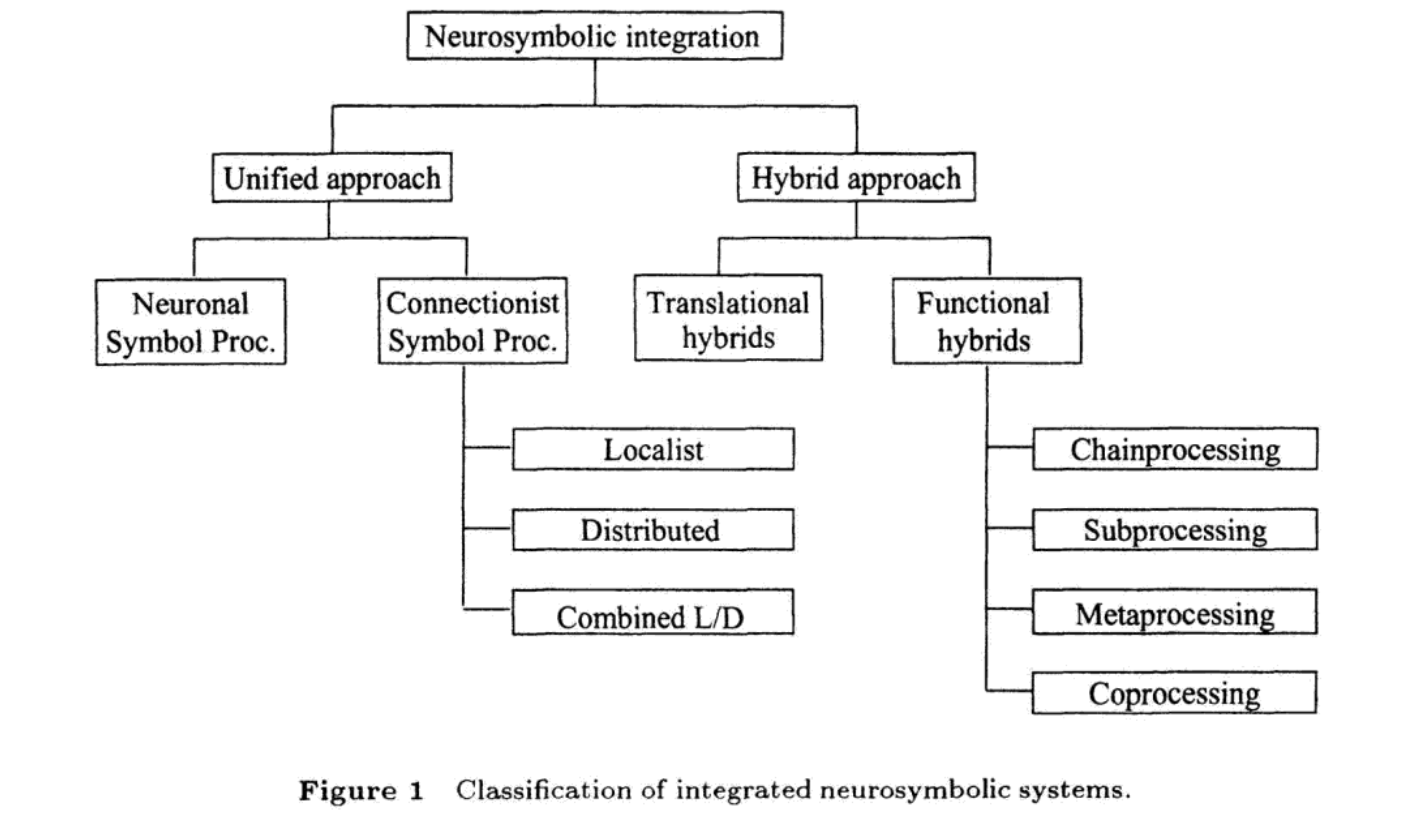
\includegraphics[width=\textwidth]{img/hybrid.png}
\end{figure}
In this distinction, \textit{unified} strategies attempt to attain neural and symbolic capabilities using neural networks, while \textit{hybrid} approaches combine neural networks with symbolic systems, such as expert systems or decision trees. We want to discuss this approach further, so we will dedicate a separate section in the following chapter on representation across symbols and neurons, after which we will have the means to consider some current directions. For now, suffice it to say that the amount of published papers on neuro-symbolic integration has seen a marked increase in the last few years, and many different perspectives have emerged.

\subsection{DCS}
As we mentioned in the introduction, attempts at integrating existing theories have been recently put forward: as an example, in 2020 Safron proposed a novel model ``Combining Integrated Information and Global Neuronal Workspace Theories With the Free Energy Principle and Active Inference Framework''\cite{safronIntegratedWorldModeling2020}.


Thanks to technical advances and renewed interest in the field, neuroscience made significant advances. Due to its biological root, when seen from an outsider's point of view its research seems more homogeneous, and even recent advances are clearly understandable. In addition, most papers published focus on narrow, specific issues and areas. This specialization of research is shared by psychology papers, but their less constrained nature makes for a more diverse array of theories, practices and explanations. In fact, if we take consciousness as a general indicator for studies in high-level cognition, a recent survey\cite{michelInformalInternetSurvey2018} on practitioners (``249 participants completed the survey, among which 80\% were in academia, and around 40\% were experts in consciousness research'') found that most perceived getting funding for it was more difficult than other subfields of neuroscience, and work that was done was perceived as less rigorous. Now, complete cognitive architectures are mostly proposed in an AI context, while past proposal from DCS are further explored and completed. In that same survey, most non-experts found the IIT (described in the last section) most promising, while overall the global workspace theory was considered the most promising. Still, the sheer amount of existing CAs makes them intractable for this document: for a complete survey, see (Ye 2018)\cite{yeSurveyCognitiveArchitectures2018}; in this paper, the CAs examined are arranged in a temporal arrangement.

\begin{figure}{h}
    \caption{Cognitive Architectures, in a temporal view\cite{yeSurveyCognitiveArchitectures2018} }
    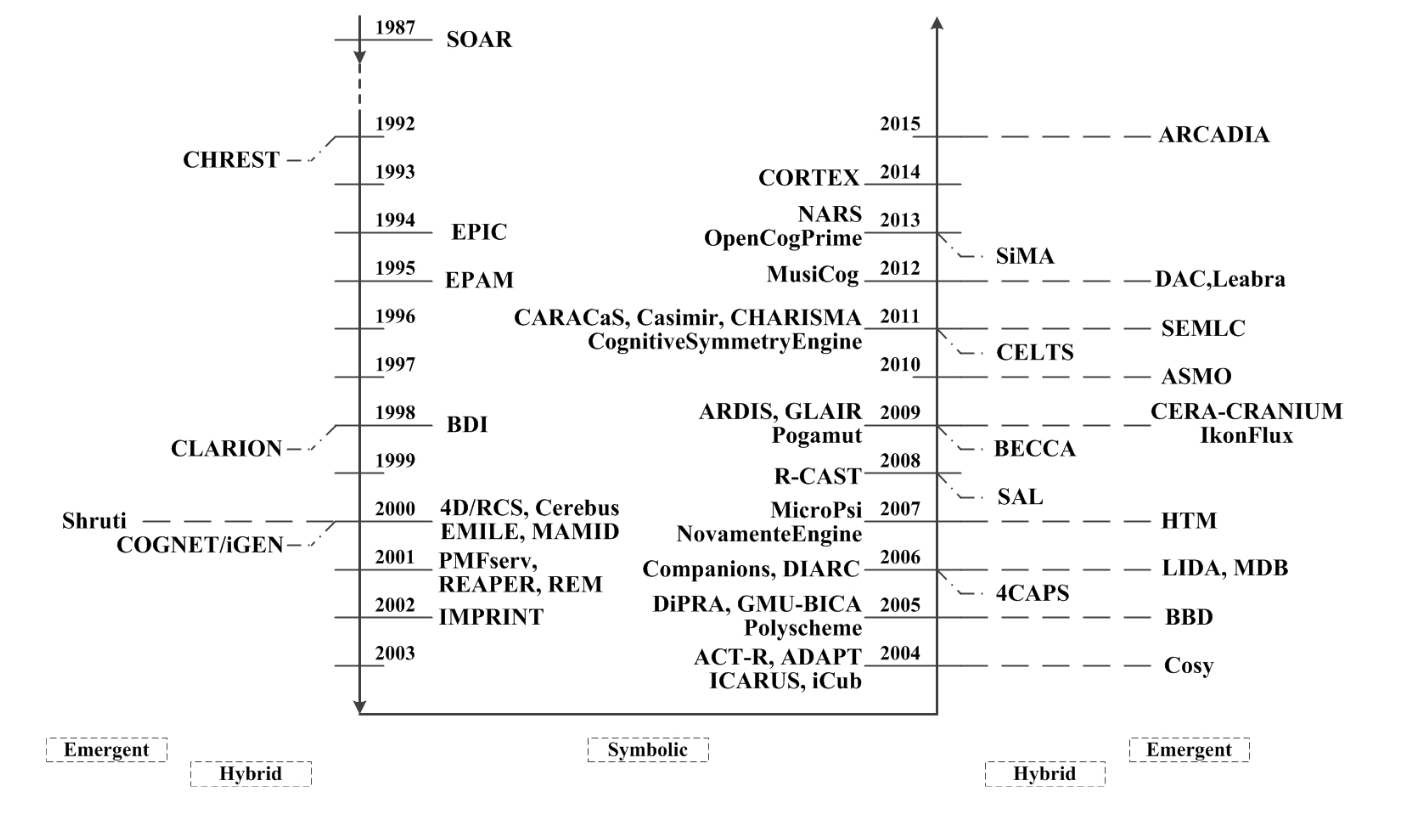
\includegraphics[width=\textwidth]{img/CAs.png}
\end{figure}

\vspace{4pt}
\textbf{Neuroscience and advances.} As we mentioned in the last section, interest in neuroscience rose significantly: the 2014 Nobel prize in Physiology or Medicine was awarded to Keef, Moser and Moser neuroscientists who discovered place and grid cells (the first are neurons that fire frequently when the subject is in a specific location in the environment, while the second are neurons that fire at regular intervals as the subject navigates an open area), although the relevant papers were published earlier\cite{okeefeDualPhaseRate2005}\cite{moserPlaceCellsGrid2008}. Large projects included the Human Connectome Project\cite{ltdNews2010}, which maps entire brains, the Brain Research through Advancing Innovative Neurotechnologies (BRAIN) Initiative\cite{NIHBRAINInitiative2013} in the US and the Human Brain Project\cite{CountdownDigitalSimulation2012} in Europe. The last interesting data point we mention is that in a bibliometric study from 2006 to 2015\cite{yeungChangingLandscapeNeuroscience2017} the most frequently reoccurring high impact yearly term was ``autism''.


\vspace{5pt}
Overall, the recent landscape of AI research is diverse, but not quite as sprawling as it has been in the past; with increase in computing power, positive results shifted from expert system to connectionist architectures, and in particulare Deep Neural Networks showing the largest results. In the next chapter, we will see how, although they may be a great tool for solving problems, they are sometimes unwieldy for \textit{understanding} problems. In this way, they have not been a panacea for understanding the brain, also due to the specific biological characteristics that are still being investigated. Nonetheless, brain research continued, with some large projects that were recently started and have yet to be completed. Psychology is, by now, more practice oriented, and neuroscience practitioners report difficulty in finding funding for consciousness research. Finally, we would like to mention three resources for academic research in AI: \href{https://distill.pub}{distill.pub}, for their incredibly clear explanations and interactive articles, \href{https://www.stateoftheart.ai}{stateoftheart.ai} for the impressive community-driven visualization of trends in research and models, and \href{https://paperswithcode.com/}{paperswithcode.com} for the always up-to-date repositories and the focus on open sourcing research.

\end{document}
